\chapter{Grundlagen}
\label{ch:grundlagen}
Das folgende Kapitel beschreibt elementare Grundlagen, die zum Verständnis der nachfolgenden Kapitel notwendig sind. Der
erste Abschnitt befasst sich mit den verwendeten Maschinen und Komponenten der Robert Bosch Packaging GmbH.

Der zweite Teil widmet sich der Künstlichen Intelligenz und den verschiedenen Untergruppen und Ausprägungen, welche in
diesem Bereich existieren. Es wird dabei unter anderem auf die Konfiguration der Produkte und Laufzeitumgebungen
eingegangen. Außerdem werden hier die Programme und Konzepzte behandelt, welche in dieser Arbeit benötigt werden.

Im letzten Teil des Kapitels folgt die Beschreibung einer Designidee bei Smartphone-Apps, allgemeine Konzepte der
Softwareentwicklung und ein Framework zum Entwickeln von Webseiten.

\section{Bosch KWE Waage}
Die Bosch KWE Serie ist ein modulares Kontrollwaagensystem, welches speziell für den Einsatz in der pharmazeutischen
Produktion entwickelt wurde. Allerdings findet es auch immer häufiger Verwendung im Bereich der Nahrungsmittel und
Süßigkeiten.

Um das Gewicht eines Produktes zu ermitteln, fahren die Produkte mit einem Förderband waagerecht über die Wiegeeinheit
der KWE.

Die KWE 4000 kann beispielsweise bei einer maximalen Leistung von bis zu 450 Pakete in der Minute eine Genauigkeit von
50mg erreichen.

Das zugehörige Display kann Produktionsstatistiken, Trendkurven und das aktuelle Gewicht des Produktes anzeigen. Durch
eigene Konfigurationen können aber auch weitere Informationen auf dem Display dargestellt werden. Auf der
Herstellerseite\cite{online_grundlagen_boschkwe} sind weitere Informationen zur aktuellen KWE-Serie einzusehen.

Die Abbildung~\ref{fig:grundlagen_boschkwe} auf Seite~\pageref{fig:grundlagen_boschkwe} zeigt eine aktuelle KWE 3000 mit
ihrem grundsätzlichen Aufbau und dem farblichen Display.

\begin{figure}[h]
    \centering
    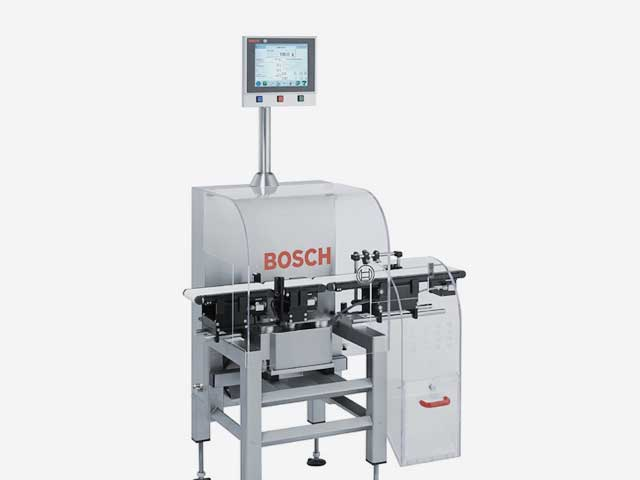
\includegraphics[scale=0.3]{images/kapitel_2/bosch_kwe.jpg}
    \caption{Abbildung einer Bosch KWE 3000}
    \label{fig:grundlagen_boschkwe}
\end{figure}

\section{Bosch Siegelmaschine}
Was ist das? Vertikale Form-, Füll- und Schließmaschinen (VFFS)
\colorbox{yellow}{Hier fehlt was}

\section{Künstliche Intelligenz}
Was ist künstliche Intelligenz?

\colorbox{yellow}{Hier fehlt was}

In Abbildung~\ref{fig:grundlagen_artificialintelligence} auf Seite~\pageref{fig:grundlagen_artificialintelligence} ist
die Einordnung der Künstlichen Intelligenz in ihre Untergruppen ersichtlich. Dabei handelt es sich um eine eigene
Darstellung frei nach CodesOfInterest\footnote{https://codesofinterest.com/2016/11/difference-artificial-intelligence-machine-learning-deep-learning.html}.

\begin{figure}[h]
    \centering
    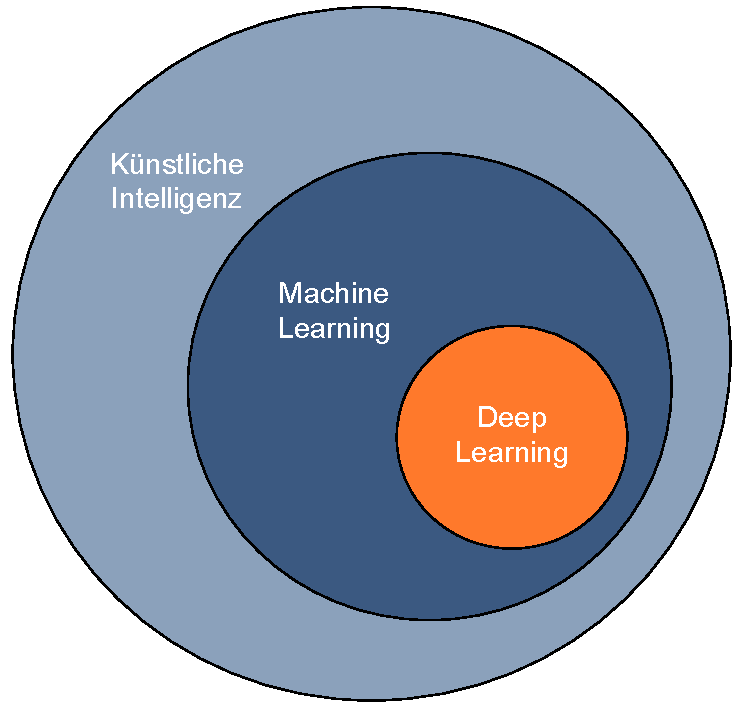
\includegraphics[scale=0.6]{images/kapitel_2/kuenstliche_intelligenz.pdf}
    \caption{Unterscheidung der Künstlichen Intelligenz}
    \label{fig:grundlagen_artificialintelligence}
\end{figure}

\section{Machine Learning}
Was ist Machine Learning?
\colorbox{yellow}{Hier fehlt was}

\subsection{Algorithmen}
Welche Algorithmen gibt es dafür
\colorbox{yellow}{Hier fehlt was}

\subsection{Bewertungskriterien}
Welche Bewertungskreterien gibt es
\colorbox{yellow}{Hier fehlt was}

\subsection{Klassifikation}
Welche Klassifikationen gibt es
\colorbox{yellow}{Hier fehlt was}

\subsection{Deep Learning}
Was ist Deep Learning
\colorbox{yellow}{Hier fehlt was}

\subsection{Neuronale Netze}
Was ist ein Neuronales Netz
\colorbox{yellow}{Hier fehlt was}

\section{Cloud}
Für Cloud Computing hat sich die Kurzform Cloud etabliert. Dies versteht das Zusammenspiel von mehreren Servern in einem
Verbund. Diese Server übernehmen zum Beispiel Aufgaben wie etwa die Datenspeicherung oder komplizierte Programmabläufe.
Dabei ist für den Cloud-Nutzer nicht ersichtlich, wie viele Server in dieser Cloud stecken oder wo diese sich befinden.

Auch wenn ein Server in diesem Gesamtsystem ausfällt, hat dies keine Auswirkungen auf das gesamte System, da die Anfragen
und Aufgaben auf andere Systeme umgeleitet werden.

Durch NIST~\cite{online_grundlagen_cloud_nist} und~\cite{online_grundlagen_cloud_computing} zeichnet sich die Cloud durch
fünf wesentliche Eigenschaften aus:

\begin{itemize}
    \item \textbf{On-Demand Self Service} \\
    Registrierte Nutzer können Resourcen selbstständig instantiieren und konfigurieren.
    \item \textbf{Broad Network Access} \\
    Der Zugriff kann von verschiedenen Endgeräten erfolgen.
    \item \textbf{Resource Pooling} \\
    Alle Resourcen des Anbieters werden gebündelt und nach Bedarf den Nutzern zugewiesen.
    \item \textbf{Rapid Elasticity} \\
    Kapazitäten können nach Bedarf skaliert werden und stehen schnell und dynamisch zur Verfügung.
    \item \textbf{Measured Service} \\
    Es existiert eine automatische Kontrolle der Ressourcen durch einen Zähler, welcher die Transparenz für den
    Anbieter und den Benutzer ermöglicht.
\end{itemize}

Auf dem Markt existieren zahlreiche Cloud-Anbieter. Im folgenden wird auf drei der Top 10 größten Anbieter und deren
Lösungen im Bereich künstliche Intelligenz eingegangen (siehe hierzu~\cite{online_grundlagen_cloud}).

\subsection{Microsoft Azure}
Azure ist die Cloud-Computing-Plattform von Microsoft. Sie ist hoch skalierbar und wendet sich mit ihren Services
hauptsächlich an Unternehmen und Entwickler. Offiziell ist Azure seit 2010 verfügbar. Seitdem erscheinen in regelmäßigen
Abständen neue Services und Funktionen.

Nutzer der Plattform können Services aus den Bereichen Infrastructure as a Service (IaaS), Platform as a Service (PaaS)
und Software as a Service (SaaS) nutzen. Auch Datenbanken, Storagesysteme sowie virtuelle Maschinen, SQL-Datenbanken und
VPN-Gateways werden bereitgestellt.

Microsoft hat sich mit ihrer Platform Azure das Ziel gesetzt, Anwendern eine flexible Cloud-Infrastruktur zur Verfügung
zu stellen, die sich den individuellen Anforderungen schnell anpassen lässt und den Betrieb einer eigenen IT-Infrastruktur
überflüssig macht.

Dank weltweit betriebener Rechenzentren stehen die Dienste mit einer hohe Verfügbarkeit auf jedem Kontinent zur Verfügung.

Microsoft Azure ermöglicht den Einsatz von Hybrid-Systemen, bei denen nur ein Teil der Services in die Cloud verlagert
und der Rest auf lokalen Servern betrieben wird. Dienste von Drittanbietern bietet ein eigener Azure Marktplatz an
(mehr unter~\cite{online_grundlagen_azure}).

\subsubsection{Azure Machine Learning Studio}
Microsoft Azure Machine Learning Studio ist ein Tool mit dem Vorhersageanalysen erstellt, getestet und bereitgestellt
werden können. Dabei ist es für die Zusammenarbeit mittels Drag \& Drop konzipiert.

Die erstellten Modelle können als Webdiest zur Verfügung gestellt werden. Andere oder auch eigene Anwendungen können
diesen Webdienst mittels HTTP-Anfragen ansprechen und nutzen (siehe dazu~\cite{article_grundlagen_azure_studio}).

\subsection{Amazon Web Services}
AWS ist eine Tochterfirma von Amazon.com. und bietet eine umfangreiche Plattform für Cloud Computing Services. Genau
wie in Microsoft Azure können dort Services für Infrastucture as a Service (IaaS), Platform as a Service (PaaS) und
Software as a Service (SaaS) genutzt werden.

Im Bereich IaaS haben Nutzer Zugrifff auf Datenspeicherung oder Rechenleistung. Über PaaS haben sie zugriff auf
Services zur einfachen Entwicklung von Webanwendungen. Bei SaaS existiert ein Katalog für Softwareanwendugnen von
externen Dienstleistern.

Ein bekanntes Beispiel für SaaS ist Google Docs, das eine standortunabhängige und Browserunabhängige Bearbeitung von
Dokumenten ermöglicht.

Public Clouds sind für Unternehmen nützlich, um beispielsweise schnell und einfach individuelle Anwendungen entwicklen
zu können ohne notwendige Produktlizenzen anderswoe erwerben zu müssen.

AWS stellt Entwicklern eine maßgeschneiderte und zuverlässige IT-Infrastruktur auf Abruf zur Verfügung (= Self Service)
(mehr über AWS unter~\cite{online_grundlagen_aws}).

\subsubsection{Amazon Machine Learning}
Amazon Machine Learning ist ein Service innerhalb von AWS. Es bietet Visualisierungstools und Assistenten die den Aufbau
von Maschin Learning-Modellen (ML) unterstützen, ohne dabei komplexe Algorithmen oder Technoligien vorauszusetzen.

Nach dem Aufbau und dem training der Modelle können diese über eine REST-API anderen Anwendungen zugänglich gemacht
werden, ohne sich dabei selbst um Infrastrukturen kümmern zu müssen.

Der Service nutzt leistungsstarke Algorithmen um ML-Modelle zu erstellen, indem er in den vorhandenen Daten automatisch
und selbstständig nach Mustern sucht. Anschließend werden diese Modelle dazu genutzt, um neue Daten zu verarbeiten und
Prognosen für eigene Anwendung zu generieren.

Der Service ist hochgradig Skalierbar und kann Milliarden Prognosen pro Tag generieren um diese in Echtzeit mit der
eigenen Anwendung zu teilen (mehr dazu in der Dokumentation~\cite{online_grundlagen_aws_learning}).

\subsection{IBM Cloud (ehemals Bluemix)}
Die IBM Cloud (ehemals Bluemix genannt) ist die von IBM entwickelte Cloud Platform. In dieser sind mehr als 160 Services
inbegriffen um zum Beispiel mobile Apps oder Webanwendungen zu entwickeln. Weiter existieren zahlreiche Analysewerkzeuge
sowie Services von Drittanbietern.

Mit Watson Analytics lassen sich beispielsweise intelligente Systeme realisieren, die Daten kognitiv (also selbstlernend,
ohne für die Problemlösungen programmiert zu sein) auswerten und für die Entscheidungsfindung aufbereiten.

Die IBM Cloud unterstützt diverse schon integrierte DevOps-Dienste, um Cloud-Anwendungen zu erstellen, auszuführen,
bereitzustellen und zu verwalten. Die Platform basiert auf der Cloud Foundry Technologie und läuft auf IBMs
Softlayer Infrastruktur.

Sie unterstützt zahlreiche Programmiersprachen, einschließlich Java, Node.js, Go, PHP, Python, Ruby Sinatra, Ruby on
Rails und kann auch andere Sprachen wie Scala durch den Einsatz von Buildpacks unterstützen~\cite{book_grundlagen_bluemix}.

Weitere Informationen üer Bluemix finden sich auf der Webseite\footnote{https://bluemix.net} und in der Dokumentation.

\subsubsection{Watson Studio}
Watson Studio ist eine SaaS-Lösung der IBM Cloud und für die Erstellung, das Trainieren und das Verwalten von trainierten
Modellen zuständig. Diese Modelle werden, ähnlich denen von Microsoft Azure und AWS, über Drag \& Drop eingerichtet
und Versioniert.

Es bietet eine vielzahl von Anwendungen für die Verarbeitung von Daten und kann mit mehreren Endnutzern gleichzeitig
genutzt werden. In Watson Studio können Modelle erstellt, trainiert und verifiziert werden (mehr hierzu
unter~\cite{online_grundlagen_watson_studio}).

\subsubsection{Cloud Object Storage}
Der Service Cloud Object Storage ist für die Speicherung von unstrukturierten Daten in der Cloud zuständig. Dieser kann
sehr einfach erweitert werden um neuen Bedürfnissen gerecht zu genügen.

Die Architektur speichert und managed die Daten über Objekte. Dies hat einen großen Vorteil gegenüber der herkömmlichen
Speicherung über Blöcke und Volumes auf Festplatten. So finden sich alle Informationen, welche einen Datenstamm zugehörig
sind, an einer einzelnen Stelle. Diese Objekte können anschließend sehr einfach kopiert, erweitert oder entfernt werden.

Jedes Objekt hat eine globale und eindeutigen Identifierierung (ID) über die es gefunden werden kann. Außerdem enthält
ein Objekt Metadaten für eine Indezierung (mehr dazu unter~\cite{book_grundlagen_objectstorage}).

\subsubsection{Apache Spark}
Bei Apache Spark handelt es sich um ein Framework, welches unter der Open-Source-Lizenz verfügbar ist. Es ist ein Projekt
der Apache Software Foundation\footnote{https://www.apache.org} und entstand aus einem Forschungsprojekt der University
of California in Berkeley \footnote{https://www.berkeley.edu}.

Apache Spark ermöglicht es, Datenabfragen und große Datenmengen aus unterschiedlichen Quellen in hoher Geschwindigkeit
und guter Perform auszuführen. Dabei wird eine verteilte Architektur und Cluster Computing genutzt.

Viele große Unternehmen unterstützen die Weiterentwicklung von Apache Spark
(mehr dazu unter~\cite{book_grundlagen_apachespark}).

\subsubsection{API Connect}
Mit dem Service IBM API Connect können alle vier Aspekte eines API-Lebenszyklusses abgebildet werden: die Erstellung, die
Ausführung, das Management und der Schutz einer eigenen API.

Mit diesem Services ist es möglich eine eigene API über ein Drag \& Drop Interface zu definieren und einzurichten. Die
so erstellte Schnittstellen kann anschließend einfach über einen Webdienst zur Verfügung gestellt werden. Dabei ist es
möglich verschienede Routen und Endpunkte zu definieren sowie die Schutzmaßnahmen und eventuelle Zugangsverwaltung
einzurichten (mehr in der Dokumentation~\cite{book_grundlagen_apiconnect}).

\subsubsection{Toolchain}
Bei einer Toolchain handelt es sich um ein Programm zur Verwaltung von Entwicklung, Bereitstellung sowie Überwachung
einer Anwendung. Verschiedene Services stehen nach der Einrichtung der Toolchain zur Verfügung. So ist es anschließend
zum Beispiel möglich, eine Integration von vorhandenen GitHub-Projekten einzubauen.

Nachdem eine eingerichtete Toolchain mit einem Git-Repository verbunden wurde kann der Quelltext gebaut und auf einem
System installiert werden. Das Git-Repository kann entweder auf einem externen Service bereitstehen oder ein IBM internes
GitLab Projekt sein.

Bei der Toolchain handelt es sich unter anderem um ein \textit{Continuous Integration}-Tool (kurz CI)
(Mehr unter~\cite{online_grundlagen_toolchain}).

\section{TensorFlow.js}
TensorFlow ist eine Deep Learning Bibliothek welche von Google entwickelt wird. Die Bibliothek wird unter der freien
Apache 2.0 Lizenz vertrieben und ist sowohl unter allen gängigen Betriebssystemem lauffähig als auch bei den meisten
Cloud-Anbietern. Diese stellen entweder aktuelle Cloud Foundry-Container bereit oder eigene Python-Container.

TensorFlow ist der Nachfolger von Googles erstem Deep Learning Tool \enquote{DistBelief}, welcher wiederum aus
\enquote{Google Brain} hervorging. Uhrsprünglich wurde es zur Erkennung von Objekten auf Fotos und Videos entwickelt.

Die Berechnungen von neuronale Netzen können durch TensorFlow auf verteilte Computersysteme geschehen. Dies ist möglich,
da diese intern durch Graphen repräsentiert werden.

Aktuell wird es für Predictive Analytics, Fraud Detection oder auch als Recommendation Engine bei Google und vielen
anderen Firmen verwendet.

In der neuesten Version lässt sich TensorFlow ohne großen Aufwand in Python integrieren. Dadurch können neue Lösungen
einfach zur Verfügung gestellt werden (mehr unter~\cite{book_grundlagen_tensorflow}).

Mittlerweile existiert eine mobile Lösung, die TensorFlow.js Bibliothek. Diese ist in jedem gängigen Browser oder auch
in Node.js lauffähig und macht schnelle \enquote{On the Edge}- sowie Offline-Vorhersagen möglich.

\section{Angular}
Bei Angular handelt es sich um ein von Google entwickeltes JavaScript-Framework. Es zielt auf die Entwicklung von
Web-Anwendungen ab und legt großen Wert auf Struktur und Qualität.

Mit seinem großen Fokus auf Architektur, Testing und isolierten Komponenten ist es für große Enterprise Anwendungen
bestens geeignet. Dabei war es das erste JavaScript-Framework das diesen Fokus hatte.

Durch Methoden wie Dependency Injection und ein ausgereiftes Tooling ermöglicht es effiziente und wartbare
Softwareentwicklung auf Basis von JavaScript (mehr unter~\cite{book_grundlagen_angular}).

\subsection{Model-View-Controller}
Die Programmarchitektur Model-View-Controller (kurz MVC) wurde um 1978 von Xerox entwickelt. Dabei wird eine
Anwendungskomponente in drei Teile zerlegt. In das oberflächenunabhängige \textit{Model}, das für die
Ausgabe zuständige \textit{View} und den für die Interpretation von Eingabeereignissen zuständigen \textit{Controller}.

Der Controller ist in dieser Architektur die Steuerungseinheit. Das Model beherbergt den Anwendungskern und die View
die Dargestellten Komponenten auf der Web-App.

Ein Controller zusammen mit einer View wird hier auch als eine Oberfläche bezeichnet. (mehr hierzu
unter~\cite{book_grundlagen_mvc}).

Es gibt zahlreiche Frameworks, welche das MVC-Patern umsetzen. Angular ist einer der bekanntesten Vertreter.

\subsection{Angular-Material}
Material Design ist eine von Google entwickelte Designsprache. Durch diese werden die Gestaltungsregeln des klassischen
Grafik-Designs mit den Möglichkeiten digitaler Benutzeroberflächen verbunden. Ziel ist es unter anderem die Verbesserung
von Benutzeroberflächen zu ermöglichen.

Material Design hat einen charakteristischen Look der es ermäglicht verschiedene Interfaces, welche im Material Design
gehalten sind, einfach zu kombinieren (mehr dazu~\cite{online_grundlagen_materialdesign}).

Die JavaScript Library \textit{Angular-Material} ermöglicht eine leichte integration des Material Designs in eine
Angular-Anwendung.

\subsection{ngx-restangular}
Mit der JavaScript-Library ngx-restangular können HTTP-Anfragen an REST-Schnitt\-stellen vereinfacht werden. Dabei
ermöglicht die Library vereinfacht Anfragen mittels den HTTP-Typen \textit{GET}, \textit{POST}, \textit{DELETE} und
\textit{UPDATE} zu stellen (mehr auf der betreffenden GitHub-Seite~\cite{online_grundlagen_restangular}).

\subsection{Observable}
Ein Observable ist das zentrale Konzept in Reactive Programming mit ReactiveX\footnote{http://reactivex.io}. Ein
Observable repräsentiert eine Menge von Daten, die in einer noch nicht bekannten Menge zu einem noch nicht bekannten
Zeitpunkt bereitstehen werden.

Ein Observer abonniert ein Observable und damit die später ankommenden Daten. Ein Obserable kann gefiltert, gruppiert
oder transformiert werden. Auch Berechnungen sind dabei möglich (mehr unter~\cite{book_grundlagen_observable}).

\subsection{Promise}
Bei Promises handelt es sich um eine Weiterentwicklung von Callbacks. Dabei helfen sie die Arbeit mit asynchronem Code
zu vereinfachen, indem sie asynchrone Operationen kapseln.

Sie zwängen asynchrone Operationen in eine einheitliche API, können verarbeitet werden bevor die Operation abgeschlossen
ist und es gibt zahlreiche Möglichkeiten Promises zu kombinieren oder in Sequenzen zu verwenden (mehr
in~\cite{book_grundlagen_promises} oder unter Matt Greer\footnote{http://www.mattgreer.org/articles/promises-in-wicked-detail}).

\subsection{flex-layout}
Bei flex-layout handelt es sich um ein Angular-Plugin, welches die Flexbox
CSS\footnote{https://www.w3schools.com/css/css3\_flexbox.asp}-Library implementiert.

Es hilft dabei, Webseiten auf verschiedene Browsergegebenheiten anzupassen. Dazu zählt unter anderem die Größe des
Displays oder die verwendete Version. Das Plugin hilft bei der Erstelltung von responsiven Webseiten (mehr auf der
GitHub-Page~\cite{online_grundlagen_flexlayout}).

%% TODO Hier gehts weiter

\section{REST}
REST-API steht für Representational State Transfer - Application Programming Interface. Diese Interfaces machen den
Austausch von Informationen uüber unterschiedliche Systeme möglich. Im Zeitalter verteilter Systeme und Cloud-Computing
trifft man oft auf unterschiedliche Systeme, welche den Einsatz von REST-API notwendig machen.

Man spricht bei REST-API auch von der Maschine-Maschine-Kommunikation, da die verschiedenen Systeme und Geräte
zusammengebracht werden und gewissermaßen die gleiche Sprache sprechen.

Mit REST-API ist es möglich geworden, Informationen und Aufgaben auf verschiedene Systeme zu verteilen und diese mit der
Hilfe von HTTP-Requests anzufordern. Jeder HTTP-Request setzt sich aus dem Endpoint und den entsprechenden Parametern
zusammen~\cite{online_grundlagen_rest}.

\section{Cloud Foundry}
Cloud Foundry ist eine Open Source Platform as a Service (PaaS) Lösung. Mit Hilfe von Cloud Foundry können Entwickler
ihre Anwendungen bauen, hochladen und ausführen. Ein großer Vorteil von Cloud Foundry ist die nahezu grenzenlose
Skalierbarkeit~\cite{book_grundlagen_cloudfoundry}.

Die Skalierbarkeit wird durch die Container-Architektur erreicht. Jeder Container beinhaltet eine eigene Anwendungsinstanz.
Dabei wird sowohl eine horizontale als auch eine vertikale Skalierung unterstützt.

Bei der horizontalen Skalierung werden zusätzliche Container gestartet oder gestoppt und ein Load Balancer vor die
Container geschaltet. Bei der vertikalen Skalierung werden jeder Instanz individuell z.B. mehr oder weniger Arbeitsspeicher
zugeteilt.

Jede Cloud Foundry Instanz besitzt eine IPV4-Adresse wodurch es mittels A-Record (Zuordnung eines DNS-Namens zu IP-Adresse)
möglich ist, eine eigene Domain mit der Anwendung zu verknüpfen.

\section{Version Control (Git)}
Git ist ein verteiltes Versionierungssystem welches frei als Open-Source zur Verfügung gestellt wird. Einige bekannte
Namen wie der Linux-Kernel, Eclipse oder Android verwenden Git für die Verwaltung ihrer Projekte.[1] Ähnlich zu
Subversion (SVN) wird Git für die Versionskontrolle (stetige Protokollierung von Änderungen) von Dateien eingesetzt. Im
Gegensatz zu SVN gibt es jedoch einige grundlegende Unterschiede, andere Begriffe und Schemata können aber auch direkt
umgelegt werden (mehr unter~\cite{book_grundlagen_git}).

\section{Node Package Manager (npm)}
Unter NPM (Node Package Manager) versteht man ein Paketmanager für node.js. Mit NPM lassen sich unter anderem
Software-Pakete für die Entwicklung von Webprojekten verwalten und steuern. Mehrere tausend OpenSource-Pakete lassen sich
unter dem Namen npm Registry bzw. npm Open Source finden und verwenden (mehr unter~\cite{book_grundlagen_npm}).

\section{Mockups}
Ein Mockup kommt während der Planung eines Webauftritts zum Einsatz. Mit der Hilfe eines Mockups kannst du deine neue
Website sehr schnell und einfach visualisieren und erhälst einen ersten Eindruck von der Gestaltung und den
Funktionalitäten deiner Website. Dazu brauchst du nicht eine Zeile Quellcode schreiben, da Mockups entweder auf Papier
entworfen oder über sogenannte Mockup-Tools am PC realisiert werden.

Bei einem Mockup tritt das Design der Website in den Hintergrund. Hier geht es einzig und alleine darum, die
verschiedenen Elemente deiner Website anzuordnen und somit einen optimalen Userflow zu realisieren. Im Fokus steht
dabei die Planung der Interaktionsmöglichkeiten und Funktionen deiner Website (mehr unter~\cite{book_grundlagen_mockups}).

\section{TypeScript}
TypeScript (kurz: TS) ist ein Superset von JavaScript. Das bedeutet, TS ist ebenfalls eine Implementierung von ECMAScript,
erweitert aber JavaScript mit zusätzlichen Features. Jeder JavaScript-Code funktioniert auch in TypeScript, aber nicht
jeder TypeScript-Code funktioniert auch in JavaScript.

Wie der Name schon verrät, erweitert TypeScript JavaScript um Typings (und Annotations). Das heißt die Programmiersprache
ist Typsicher. Wie z.B. auch Java (mehr unter~\cite{book_grundlagen_typescript}).

\begin{lstlisting}[language=JavaScript, caption=Unterschied zwischen JavaScript und TypeScript, label=Unterschied zwischen JavaScript und TypeScript]
    // JavaScript
    var name = "Vorname Nachname";

    // TypeScript
    let name : string = "Vorname Nachname";
\end{lstlisting}

\section{WebView}
Bei WebView handelt es sich um ein Android- und iOS-Layout, das Webseiten darstellen kann. Über Schnitstellen werden
Informationen wie Webseite, URL und Größe üergeben. Das Laden, das Anzeigen und die Interaktion mit der Webseite üernimmt
das Layout selbstständig.

Das Layout steht sowohl unter Android als auch iOS in den frühesten Versionen zur Verfügung (Weitere Informationen
unter~\cite{online_grundlagen_webview}).